% ta med damping på DP-delle

\documentclass[aspectratio=169,xcolor=dvipsnames]{beamer}
%\usetheme{SimplePlus}

\usepackage{hyperref}
\usepackage{graphicx} % Allows including images
\usepackage{booktabs} % Allows the use of \toprule, \midrule and \bottomrule in tables

%----------------------------------------------------------------------------------------
%	TITLE PAGE
%----------------------------------------------------------------------------------------

\title[Industrielektronikk]{Industrielektronikk} % The short title appears at the bottom of every slide, the full title is only on the title page
%\subtitle{Subtitle}

\author[Fred-Olav] {Fred-Olav Mosdal}

\institute[Gand VGS] % Your institution as it will appear on the bottom of every slide, may be shorthand to save space
{
    Gand VGS \\
    VG1 TIF }
\date{\today} % Date, can be changed to a custom date


%----------------------------------------------------------------------------------------
%	PRESENTATION SLIDES
%----------------------------------------------------------------------------------------

\begin{document}
\begin{frame}
\titlepage
\end{frame}

\begin{frame}
	\frametitle{Styringsteknikk D426}

	\begin{columns}
		\begin{column}{0.5\textwidth}
			Mål:
			\begin{itemize}
				\item \url{https://www.udir.no/lk20/pin02-03}
			\end{itemize}
		\end{column}

		\begin{column}{0.5\textwidth}
			$$\includegraphics[width=0.8\textwidth]{../output/noGPLimages/udir.pdf}$$
		\end{column}
	\end{columns}
\end{frame}

\begin{frame}
	\frametitle{Fagenes relevans og sentrale verdier}

	\begin{columns}
		\begin{column}{0.5\textwidth}
			Vg2 industriteknologi handler om å utvikle kompetanse innenfor teknologiske, produksjonsrettede og utviklingsorienterte yrker. Programfagene gir en bred plattform for videre yrkesvalg innenfor bruk av ulike materialer, verktøy, teknikker og maskiner. Programfagene skal bidra til å utvikle elevene til selvstendige og omstillingsdyktige fagarbeidere innenfor yrker der programmering, robotisering og automatisering er en del av hverdagen. Programfagene skal bidra til å utvikle en helhetsforståelse av produksjonsprosesser og gi en tverrfaglig forståelse av fagområdene i arbeidslivet.
		\end{column}

		\begin{column}{0.5\textwidth}
			$$\includegraphics[width=0.8\textwidth]{../output/noGPLimages/udir.pdf}$$
		\end{column}
	\end{columns}
\end{frame}

\begin{frame}
	\frametitle{Kompetansemål:}

	\begin{columns}
		\begin{column}{0.5\textwidth}
			Mål:
			\begin{itemize}
				
				\item montere, sette i drift og feilsøke automatiserte hydraulikk- og pneumatikkanlegg etter spesifikasjoner 
				\item montere, sette i drift og feilsøke maskiner og utstyr i en produksjonsprosess
				\item planlegge og gjennomføre praktiske arbeidsoppgaver i både kjente og ukjente sammenhenger 
				\item bruke digitale verktøy til å utarbeide modeller, tegninger, skjemaer, arbeidsbeskrivelser og kvalitetssikringssystemer i planlegging og produksjon 

			\end{itemize}
		\end{column}

		\begin{column}{0.5\textwidth}
			$$\includegraphics[width=0.8\textwidth]{../output/noGPLimages/udir.pdf}$$
		\end{column}
	\end{columns}
\end{frame}
\begin{frame}
	\frametitle{Kompetansemål:}

	\begin{columns}
		\begin{column}{0.5\textwidth}
			Mål:
			\begin{itemize}
				\item utarbeide rapporter og skjemaer knyttet til arbeidsoppgaver og vurdere resultatet av eget arbeid 
				\item anvende program for simulering og styring av robot og automasjon 
				\item bruke additiv tilvirkning for å løse læringsoppdrag 
				\item utarbeide og følge sikker jobb-analyser ved farlige operasjoner i henhold til gjeldende forskrifter 
				\item arbeide på elektriske og automatiserte systemer ved reparasjons- og vedlikeholdsarbeid etter instrukser og gjeldende forskrifter

			\end{itemize}
		\end{column}

		\begin{column}{0.5\textwidth}
			$$\includegraphics[width=0.8\textwidth]{../output/noGPLimages/udir.pdf}$$
		\end{column}
	\end{columns}
\end{frame}

\begin{frame}
	\frametitle{Boken}

	\begin{columns}
		\begin{column}{0.5\textwidth}
			I styringsteknikken skal vi ha følgende kapittel:

			\begin{itemize}
			\item Kap. 11 Programmerbare logiske styringer 
			\item Kap. 12 Elektriske Anlegg 
			\item Kap. 13 Hydraulikk 
			\item Kap. 14 Pneumatikk

			\end{itemize}
		\end{column}

		\begin{column}{0.5\textwidth}
			$$\includegraphics[width=0.7\textwidth]{../output/noGPLimages/RepOgVedlikehold.jpg}$$
		\end{column}
	\end{columns}
\end{frame}

\begin{frame}
	\frametitle{Grunnkunnskaper}

	\Huge
	Grunnkunnskaper\\
\normalsize
\vskip 2 cm
Kunnskaper som må være på plass for å forstå det som kommer
\end{frame}


\begin{frame}
	\frametitle{SI-prefikser}

	\begin{columns}
		\begin{column}{0.5\textwidth}
			Mål:
			\begin{itemize}
				\item Brukes ved store eller små strørrelser 
				\item Hardisk på 2TB
				\item Prosessor med transistorstørrelse på 7nm
			\end{itemize}
		\end{column}

		\begin{column}{0.5\textwidth}
			$$\includegraphics[width=0.8\textwidth]{SIenheter.eps}$$
		\end{column}
	\end{columns}
\end{frame}





\end{document}
